%!TEX root = ../dokumentation.tex

\chapter{Das erste Kapitel}
Erste Erwähnung eines Akronyms wird als Fußnote angezeigt. Jede weitere wird
nur verlinkt: \ac{AGPL}. Zweite Erwähnung \ac{AGPL}

Verweise auf das Glossar: \gls{Glossareintrag}, \glspl{Glossareintrag}

Nur erwähnte Literaturverweise werden auch im Literaturverzeichnis gedruckt:
\cite{baumgartner:2002}, \cite{dreyfus:1980}

Meine erste Fußnote\footnote{Ich bin eine Fußnote}

\begin{wrapfigure}{r}{.4\textwidth}
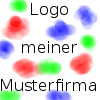
\includegraphics[height=.4\textwidth]{logo.png}
\vspace{-15pt}
\caption{Das Logo der Musterfirma\footnotemark}
\end{wrapfigure}
%Quelle muss in Fußnote stehen (da sonst aufgrund eines Fehlers nicht kompiliert
% wird)
\footnotetext{aus \cite{mustermann:2012}}
Ein ganz langer Text, der das Bild umfließt. Ein ganz langer Text, der das Bild
umfließt. Ein ganz langer Text, der das Bild umfließt. Ein ganz langer Text, der
das Bild umfließt. Ein ganz langer Text, der das Bild umfließt. Ein ganz langer
Text, der das Bild umfließt. Ein ganz langer Text, der das Bild umfließt. Ein
ganz langer Text, der das Bild umfließt. Ein ganz langer Text, der das Bild
umfließt. Ein ganz langer Text, der das Bild umfließt. Ein ganz langer Text, der
das Bild umfließt. Ein ganz langer Text, der das Bild umfließt. Ein ganz langer Text, der das Bild

umfließt. Ein ganz langer Text, der das Bild umfließt. Ein ganz langer Text, der
das Bild umfließt. Ein ganz langer Text, der das Bild umfließt. Ein ganz langer
Text, der das Bild umfließt. Ein ganz langer Text, der das Bild umfließt. Ein
ganz langer Text, der das Bild umfließt. Ein ganz langer Text, der das Bild
umfließt. Ein ganz langer Text, der das Bild umfließt. Ein ganz langer Text, der
das Bild umfließt.
